\section{Introduction}
Visual Question Answering (VQA) is an emerging interdisciplinary research problem at the intersection of computer vision, natural language processing and artificial intelligence. It has many real-life applications, such as automatic querying of surveillance video~\cite{tu2014joint} or assisting the visually impaired~\cite{lasecki2014increasing}. Compared to the recently popular image captioning task~\cite{donahue2014long,vinyals2014show,karpathy2014deep,fang2014captions}, VQA requires a deeper understanding of the image, but is considerably easier to evaluate. It also puts more focus on artificial intelligence, namely the inference process needed to produce the answer to the visual question.

\begin{figure}[!t]
\centering
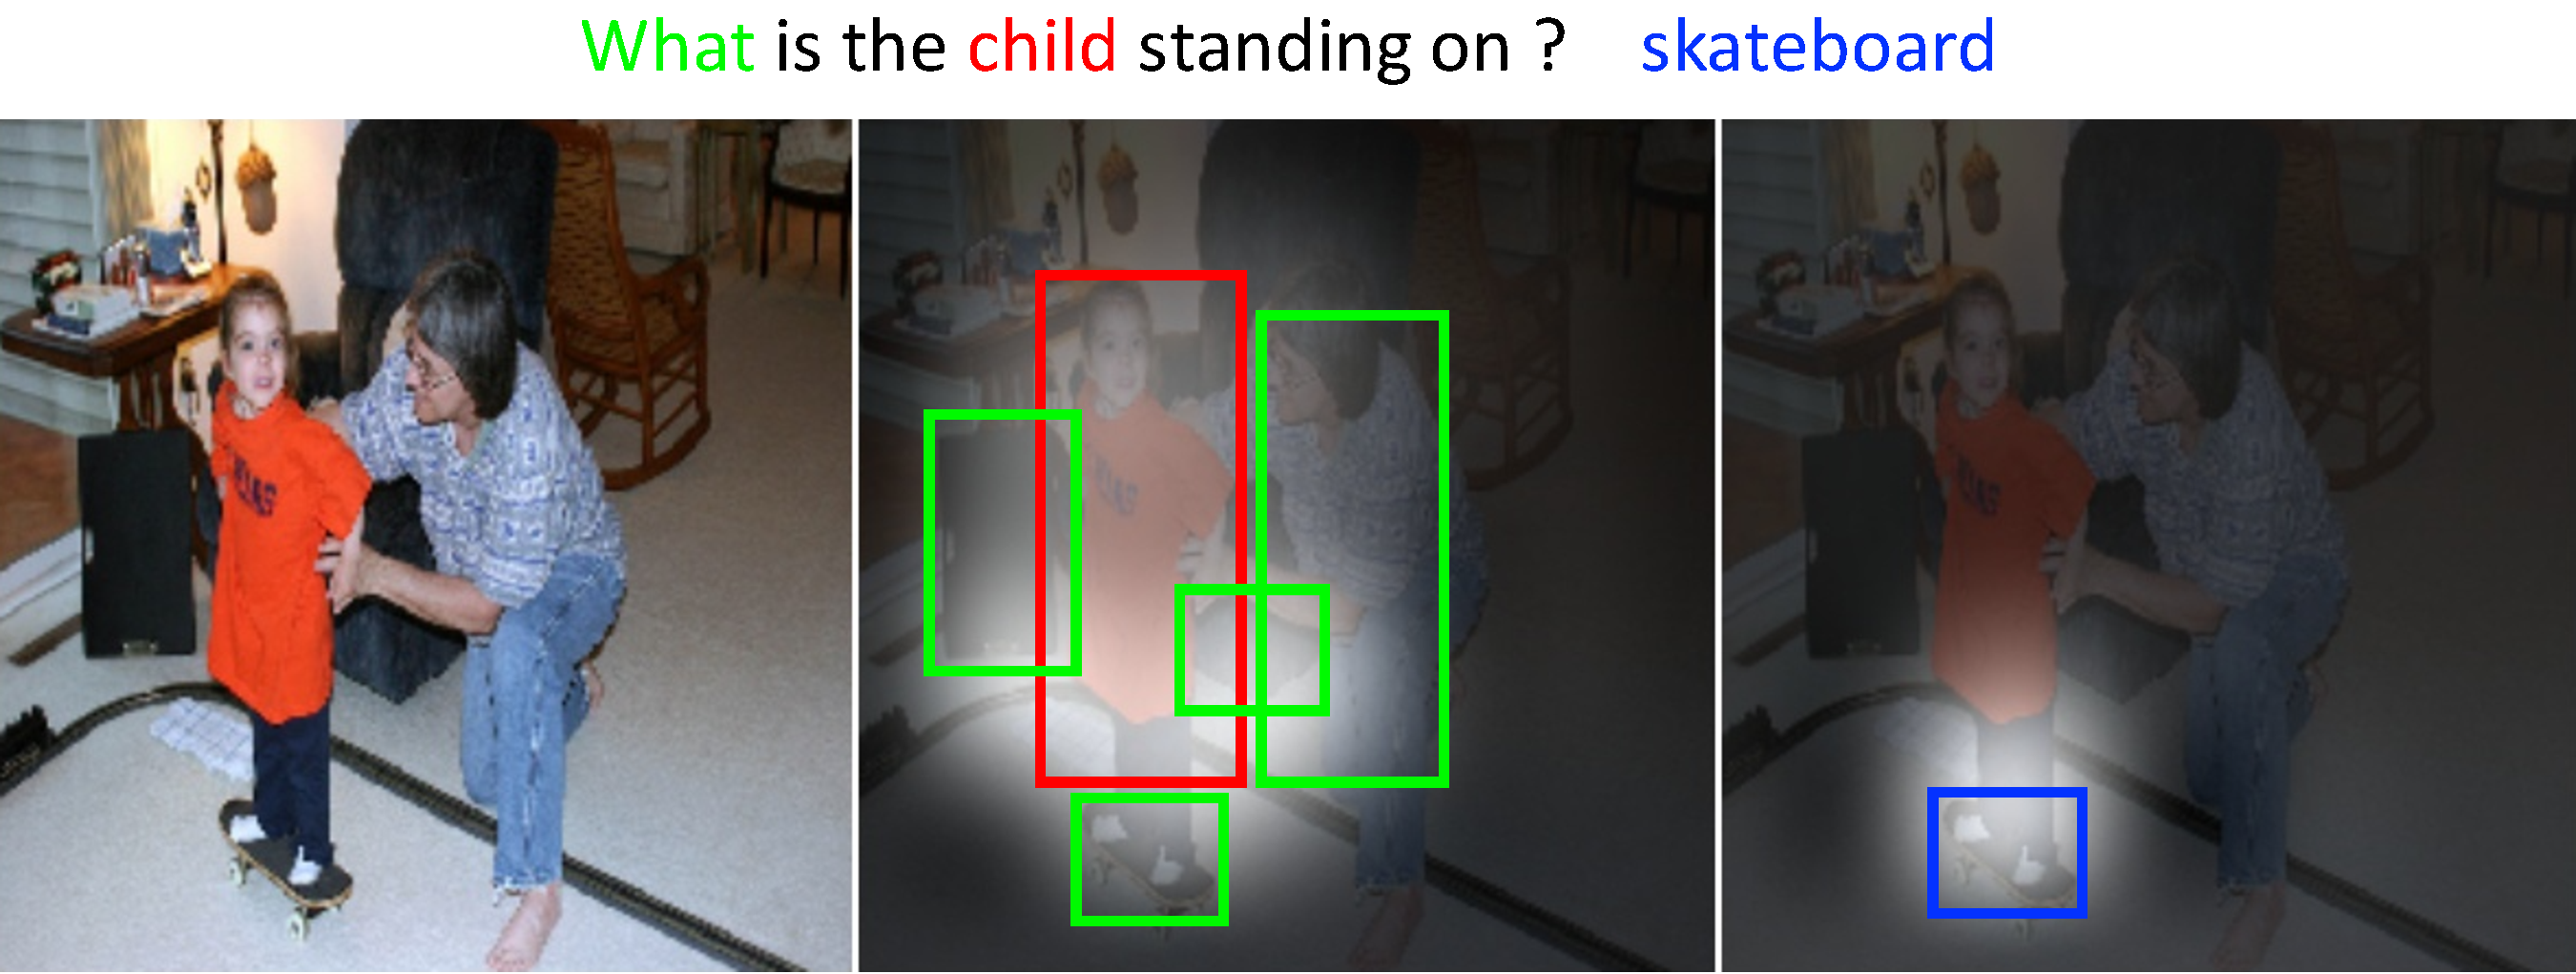
\includegraphics[width=0.7\columnwidth,height=2.6cm]{figures/concept_graph.pdf}
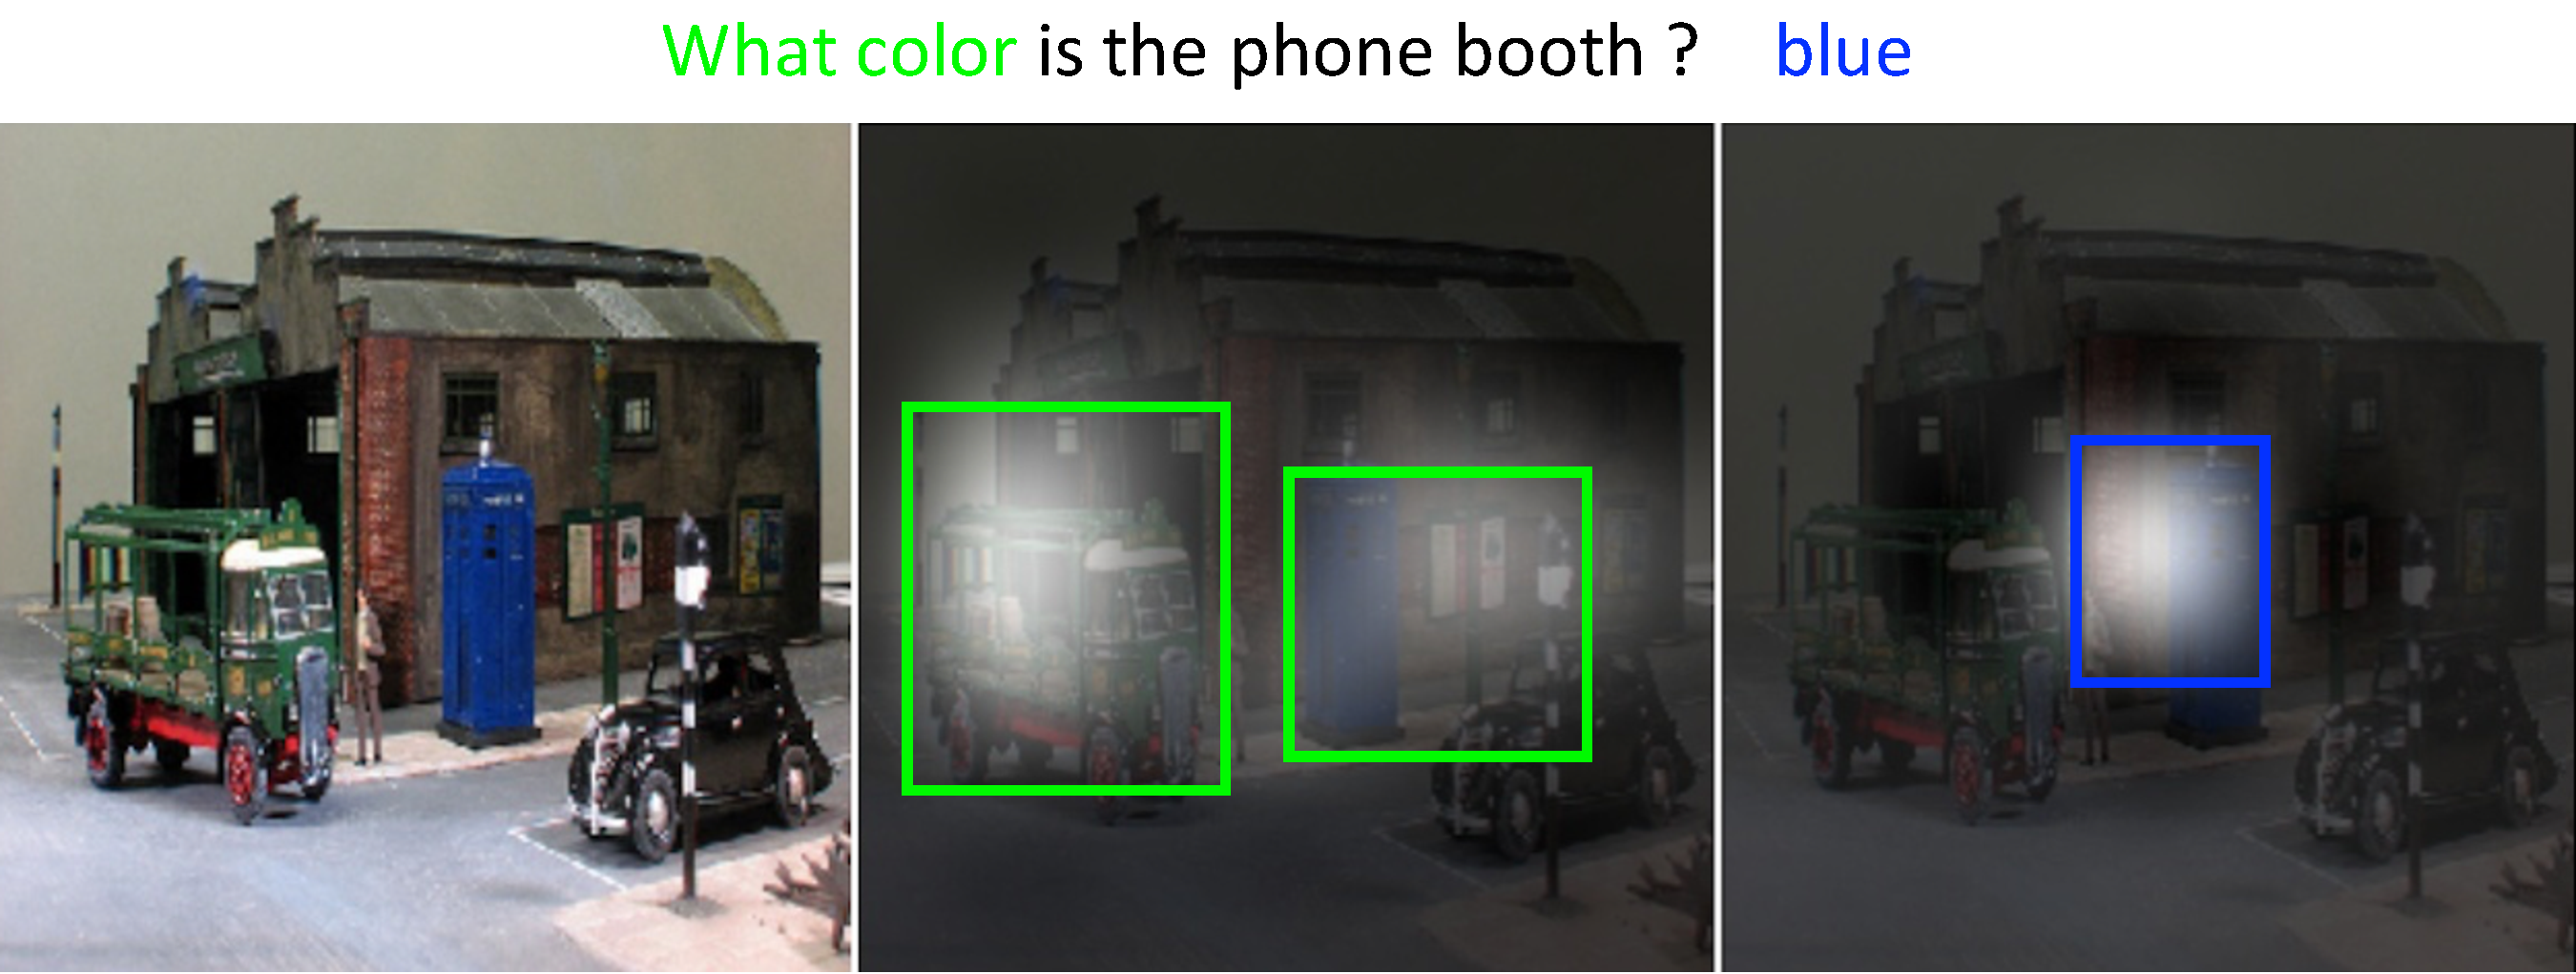
\includegraphics[width=0.7\columnwidth,height=2.6cm]{figures/concept_graph2.pdf}
\vspace{-0.1in}
\caption{We propose a Spatial Memory Network for VQA (SMem-VQA) that answers questions about images using spatial inference.
The figure shows the inference process of our two-hop model on examples from the VQA dataset~\cite{DBLP:journals/corr/AntolALMBZP15}. In the first hop (middle), the attention process captures the correspondence between individual words in the question and image regions. High attention regions (bright areas) are marked with bounding boxes and the corresponding words are highlighted using the same color. In the second hop (right), the fine-grained evidence gathered in the first hop, as well as an embedding of the entire question, are used to collect more exact evidence to predict the answer. (Best viewed in color.) }
\label{fig:concept}
\vspace{-0.2in}
\end{figure}

In one of the early works~\cite{DBLP:journals/corr/MalinowskiF14}, VQA is seen as a Turing test proxy. The authors propose an approach based on handcrafted features using a semantic parse of the question and scene analysis of the image combined in a latent-world Bayesian framework. More recently, several end-to-end deep neural networks that learn features directly from data have been applied to this problem~\cite{malinowski2015ask,DBLP:journals/corr/RenKZ15}.
Most of these are directly adapted from captioning models~\cite{donahue2014long,vinyals2014show,karpathy2014deep},
and utilize a recurrent LSTM network, which takes the question and Convolutional Neural Net (CNN) image features as input, and outputs the answer. Though the deep learning methods in~\cite{malinowski2015ask,DBLP:journals/corr/RenKZ15} have shown great improvement compared to the handcrafted feature method~\cite{DBLP:journals/corr/MalinowskiF14}, they have their own drawbacks. These models based on the LSTM reading in both the question and the image features do not show a clear improvement compared to an LSTM reading in the question only~\cite{malinowski2015ask,DBLP:journals/corr/RenKZ15}.   
Furthermore, the rather complicated LSTM models obtain similar or worse accuracy to a baseline model which concatenates CNN features and a bag-of-words question embedding to predict the answer, see the IMG+BOW model in~\cite{DBLP:journals/corr/RenKZ15} and the iBOWIMG model in~\cite{zhou2015simple}.

A major drawback of existing models is that they do not have any explicit notion of object position, and do not support the computation of intermediate results based on spatial attention.
Our intuition is that answering visual questions often involves looking at different spatial regions and comparing their contents and/or locations. For example, to answer the questions in Fig.~\ref{fig:concept}, we need to look at a portion of the image, such as the child or the phone booth.
Similarly, to answer the question ``Is there a cat in the basket?'' in Fig.~\ref{fig:illus}, we can first find the basket and the cat objects, and then compare their locations.

We propose a new deep learning approach to VQA that incorporates explicit spatial attention, which we call the Spatial Memory Network VQA (SMem-VQA). 
Our approach is based on memory networks, which have recently been proposed for text Question Answering (QA)~\cite{DBLP:journals/corr/WestonCB14,sukhbaatar2015end}. Memory networks combine learned text embeddings with an attention mechanism and multi-step inference. 
The text QA memory network stores textual knowledge in its ``memory" in the form of sentences, and selects relevant sentences to infer the answer. However, in VQA, the knowledge is in the form of an image, thus the memory and the question come from different modalities.
We adapt the end-to-end memory network~\cite{sukhbaatar2015end} to solve visual question answering by storing the convolutional network outputs obtained from different receptive fields into the memory, which explicitly allows spatial attention over the image. We also propose to repeat the process of gathering evidence from attended regions, enabling the model to update the answer based on several attention steps, or ``hops''. The entire model is trained end-to-end and the evidence for the computed answer can be visualized using the attention weights. 

To summarize our contributions, in this paper we\vspace{-0.1in}
\begin{itemize}%[noitemsep]
\item propose a novel multi-hop memory network with spatial attention for the VQA task which allows one to visualize the spatial inference process used by the deep network (a CAFFE~\cite{jia2014caffe} implementation will be made available), 
\item design an attention architecture in the first hop which uses each word embedding to capture fine-grained alignment between the image and question,
\item create a series of synthetic questions that explicitly require spatial inference to analyze the working principles of the network, and show that it learns logical inference rules by visualizing the attention weights,
\item provide an extensive evaluation of several existing models and our own model on the same publicly available datasets.
\end{itemize}


Sec.~2 introduces relevant work on memory networks and attention models. Sec.~3 describes our design of the multi-hop memory network architecture for visual question answering (SMem-VQA). Sec.~4  visualizes the inference rules learned by the network for synthetic spatial questions and shows the experimental results on DAQUAR~\cite{DBLP:journals/corr/MalinowskiF14} and VQA~\cite{DBLP:journals/corr/AntolALMBZP15} datasets. Sec.~5 concludes the paper.



